\subsection{Equal-data system comparison}

Laya LoRA has the highest 4k macro F1 point estimate in Table~\ref{tab:main}. The prespecified Laya-minus-TF-IDF contrast is 0.0199 with paired 95\% interval $[-0.0022, 0.0423]$. This interval establishes neither an advantage nor equivalence. At default decisions, Laya skips 156 additional documents but misses 80 more review-worthy references. Its review precision is 94.3\% versus 89.9\%, while recall is 82.6\% versus 87.8\%. Higher macro F1 does not imply fewer missed review-worthy references. Laya's warm mean inference latency is 64.9 times the lexical classifier's.

\begin{table}[!htbp]
\centering
\caption{Core systems on the revised 2,000-document evaluation. Default decisions; false negatives (FN) are divided by review-reference support. All trainable systems use the same 4k bodies; majority counts those labels, and SDK has no task fit. Warm inference includes full document processing.}
\label{tab:main}
\small
\setlength{\tabcolsep}{3.5pt}
\begin{tabularx}{\linewidth}{@{}Xrrrrr@{}}
\toprule
System & F1 (95\% CI) & FN & Skipped & Mean ms & P95 ms\\
\midrule
Training majority & 0.436 $[0.429, 0.441]$ & 0/1543 & 0.0\% & 2.97 & 3.45\\
Word TF-IDF/logistic & 0.764 $[0.743, 0.786]$ & 188/1543 & 24.6\% & 4.58 & 8.16\\
Frozen FinBERT/logistic & 0.718 $[0.696, 0.740]$ & 302/1543 & 30.9\% & 35.81 & 113.33\\
FinBERT LoRA & 0.743 $[0.721, 0.763]$ & 352/1543 & 36.5\% & 35.17 & 116.72\\
Laya native SDK & 0.542 $[0.519, 0.567]$ & 96/1543 & 8.3\% & 334.22 & 1332.02\\
Laya head & 0.609 $[0.587, 0.632]$ & 473/1543 & 37.3\% & 276.66 & 1131.21\\
Laya LoRA & 0.784 $[0.764, 0.805]$ & 268/1543 & 32.4\% & 297.19 & 1207.55\\
\bottomrule
\end{tabularx}
\end{table}

\begin{figure}[!htbp]\centering
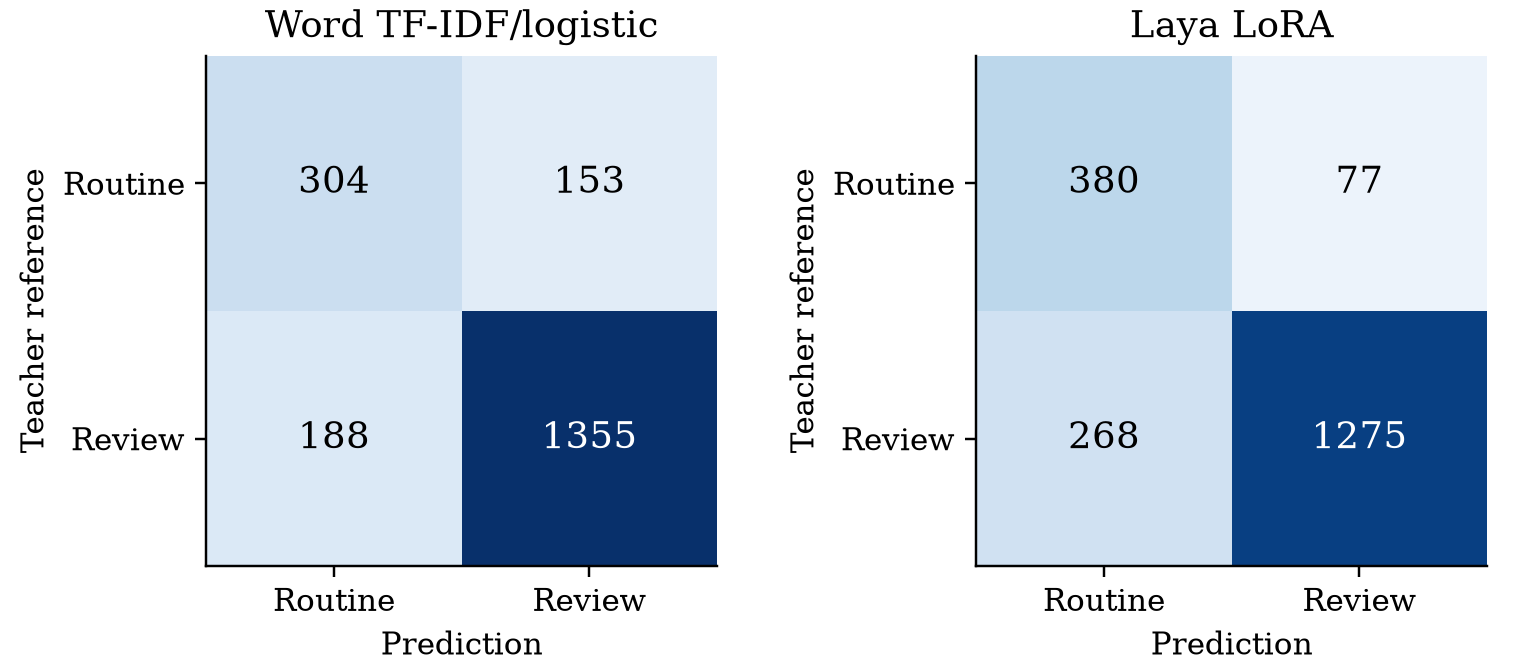
\includegraphics[width=\linewidth]{confusion.png}
\caption{Default two-class confusion matrices for the fixed primary pair. Rows are teacher references; columns are model predictions. Counts sum to 2,000 in each matrix.}\label{fig:confusion}\end{figure}

\subsection{Review workload and missed references}

Table~\ref{tab:policy} applies calibration-selected thresholds unchanged to test. The 1\% fitting target and 20\% skip budget produce different achieved workloads across systems; neither is a test guarantee. For the primary pair, the 1\% calibration miss target reduces skipped test reading to 2.5\% for Laya and 6.2\% for TF-IDF. Stringent miss control substantially reduces skipping; achieved misses must be read alongside the remaining workload.

\begin{table}[!htbp]
\centering
\caption{Achieved test outcomes for two calibration policies. The left pair uses an empirical 1\% calibration miss target; the right pair maximizes calibration skips within 20\%. All policies skip only routine predictions and preserve ties. Achieved test workloads are not assumed equal.}
\label{tab:policy}
\small
\setlength{\tabcolsep}{3.5pt}
\begin{tabularx}{\linewidth}{@{}Xrrrr@{}}
\toprule
System & 1\% miss: FN & Skipped & 20\% skip: FN & Skipped\\
\midrule
Training majority & 0/1543 & 0.0\% & 0/1543 & 0.0\%\\
Word TF-IDF/logistic & 20/1543 & 6.2\% & 95/1543 & 15.8\%\\
Frozen FinBERT/logistic & 27/1543 & 4.0\% & 159/1543 & 18.7\%\\
FinBERT LoRA & 31/1543 & 5.3\% & 144/1543 & 19.8\%\\
Laya native SDK & 14/1543 & 0.9\% & 95/1543 & 8.2\%\\
Laya head & 14/1543 & 1.4\% & 240/1543 & 19.6\%\\
Laya LoRA & 7/1543 & 2.5\% & 124/1543 & 19.7\%\\
\bottomrule
\end{tabularx}
\end{table}

\subsection{Adaptation and sample efficiency}

Figure~\ref{fig:learning} shows the nested training-size curves alongside the shared-4k comparison. Source/class composition and optimization steps also vary with size, so the curves do not isolate sample count causally. Intervals condition on fixed fitted runs and are uncorrected for multiple comparisons.

\begin{figure}[!htbp]\centering
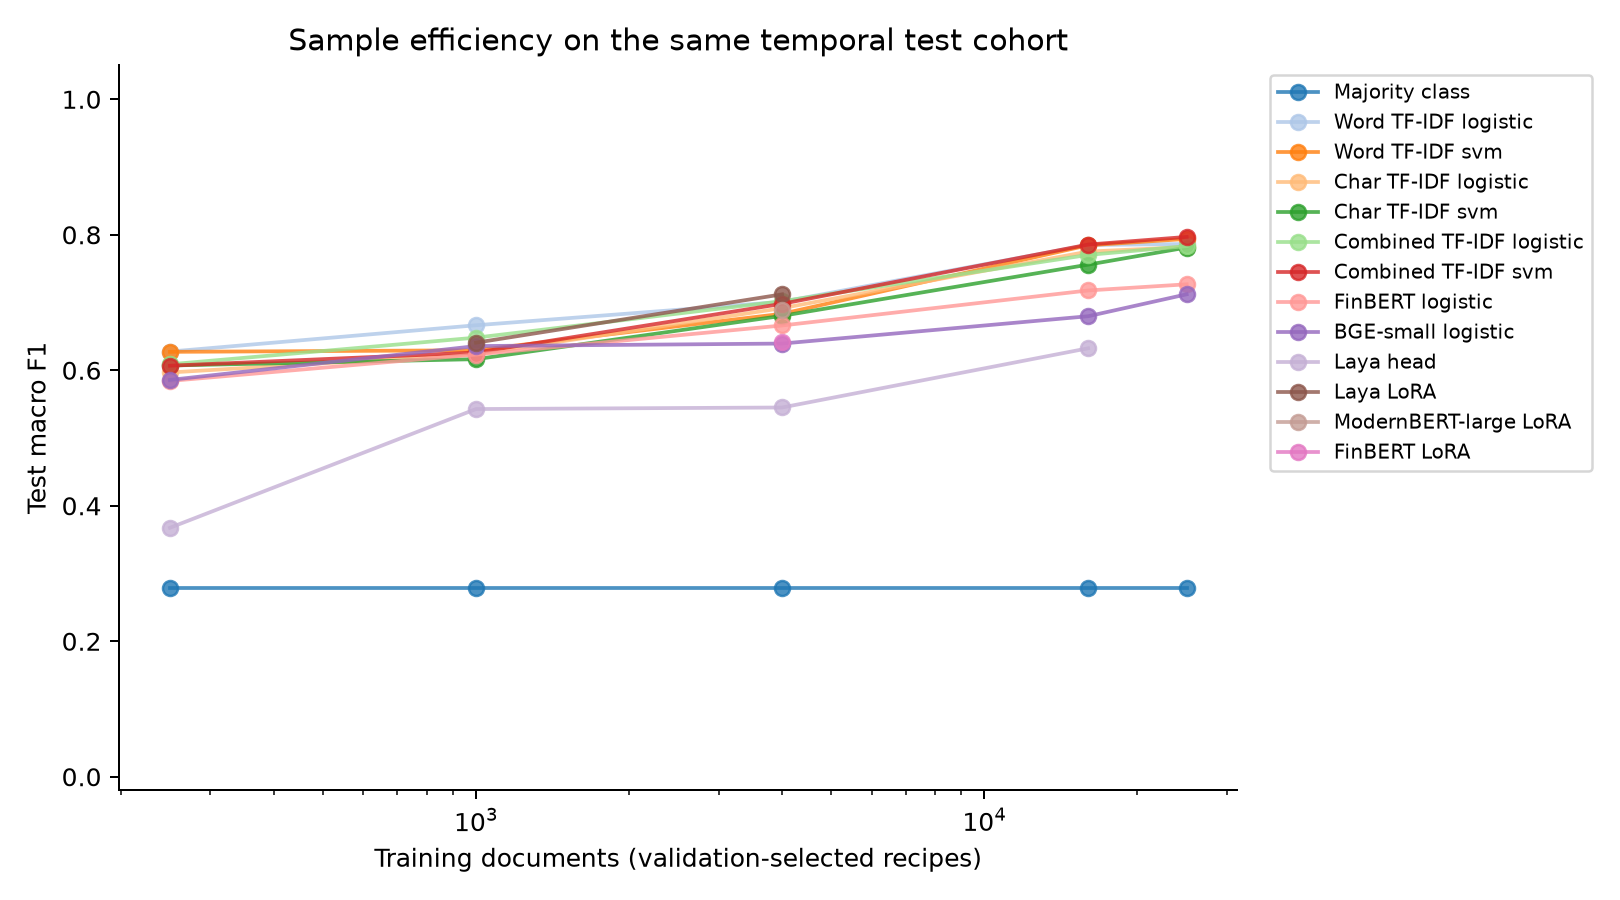
\includegraphics[width=\linewidth]{learning-curves.png}
\caption{Nested training-size curves for completed recipes. Left: macro F1. Right: review-reference miss rate at default decisions. Vertical segments are marginal whole-group 95\% intervals. LoRA curves stop at 16,000 training documents.}\label{fig:learning}\end{figure}

At 16k, Laya LoRA reaches F1 0.8424 and word TF-IDF/logistic 0.8245; FinBERT LoRA reaches 0.8140. Laya and TF-IDF default miss counts are 171 and 141, with 28.0\% and 24.3\% skipped. The successful commands take 20.66 hours and 59.5 seconds, respectively; FinBERT LoRA takes 2.51 hours. These larger-run point estimates supplement the fixed 4k primary comparison; they do not replace it.

The matched pre-update comparisons in Table~\ref{tab:controls} separate task fitting from context, pooling and initial-head differences. Each recipe is compared with its own preserved initial state. These controls do not isolate pretraining or equalize classifier budgets across model families.

The primary systems share 122 default missed references, with 146 additional Laya-only and 66 TF-IDF-only misses. This overlap describes the fixed predictions; it does not evaluate a new combined routing rule.

\begin{table}[!htbp]
\centering
\caption{Paired training-size F1 increments for fixed system families. Conditional 95\% intervals; supplementary comparisons are uncorrected.}
\label{tab:increments}
\small
\setlength{\tabcolsep}{3.5pt}
\begin{tabularx}{\linewidth}{@{}XXrr@{}}
\toprule
System & Training change & $\Delta$ F1 & 95\% interval\\
\midrule
Word TF-IDF/logistic & 4k to 16k & 0.0600 & $[0.0421, 0.0795]$\\
Word TF-IDF/logistic & 16k to 25k & -0.0145 & $[-0.0295, 0.0013]$\\
Frozen FinBERT/logistic & 4k to 16k & 0.0458 & $[0.0292, 0.0624]$\\
Frozen FinBERT/logistic & 16k to 25k & 0.0069 & $[-0.0098, 0.0230]$\\
Laya LoRA & 4k to 16k & 0.0581 & $[0.0428, 0.0735]$\\
FinBERT LoRA & 4k to 16k & 0.0715 & $[0.0535, 0.0899]$\\
\bottomrule
\end{tabularx}
\end{table}
